\documentclass[conference]{IEEEtran}
\pdfminorversion=7
\usepackage{amsmath,booktabs,graphicx,cite,balance}
\usepackage[hidelinks]{hyperref}
\newcommand{\LiveDelta}{-60.2 [-69.2, -50.8]}
\newcommand{\LiveFixed}{135/227 & 0/227}
\newcommand{\LiveGraded}{0/227 & 0/227}
\newcommand{\PolicyEffects}{%
Collateral (pp) & Graded--fixed & -49.947 [-52.000, -47.845] \\
Persistent delivery (pp) & Graded--fixed & -47.574 [-49.575, -45.184] \\
Full-host ACK (s) & Graded--fixed & 0.675 [0.583, 0.758] \\
Initial ACK (s) & Graded--fixed & -0.033 [-0.132, 0.078] \\
Install-window receipts (packets) & Guard on--off & -0.975 [-1.425, -0.575] \\
}
\newcommand{\DetectorRows}{%
AIS-default & 3517 & 10503 & 164 & 7413 & 0.560 & 0.854 & 0.399 & 0.001 \\
AIS-tuned & 3514 & 10506 & 0 & 7577 & 0.543 & 1.000 & 0.399 & 0.001 \\
TRW & 4400 & 9620 & 9 & 7568 & 0.659 & 0.964 & 0.593 & 0.000 \\
RF-tuned & 14020 & 0 & 141 & 7436 & 0.905 & 0.785 & 0.930 & 0.000 \\
Entropy & 1946 & 12074 & 75 & 7502 & 0.477 & 0.739 & 0.489 & 0.000 \\
IA-Window & 80 & 13940 & 0 & 7577 & 0.444 & 1.000 & 0.444 & 0.000 \\
}
\newcommand{\DetectorIntervals}{%
AIS-tuned & 0.543 [0.542, 0.544] & 0.533 [0.532, 0.535] & 0.000 [0.000, 0.000] \\
TRW & 0.659 [0.652, 0.665] & 0.667 [0.667, 0.667] & 0.001 [0.000, 0.002] \\
RF-tuned & 0.905 [0.882, 0.928] & 1.000 [1.000, 1.000] & 0.019 [0.014, 0.024] \\
}

% Generated from successful real-source smoke-trial metadata.
\newcommand{\ScaleSources}{200}
\newcommand{\ScalePackets}{159033}
\newcommand{\ScaleAttempts}{26485}

\newcommand{\InferenceRows}{%
Install-window receipts (pkts) & Graded$-$fixed & 0.075 [-0.325, 0.425] & 0.863 & 0.09 & 5/5/10 & 0.450 & 1.000 \\
Install-window receipts (pkts) & Guard on$-$off & -0.975 [-1.425, -0.575] & 1.006 & -0.97 & 16/3/1 & $<$0.001 & 0.004 \\
Collateral loss (pp) & Graded$-$fixed & -49.947 [-52.000, -47.845] & 4.957 & -10.08 & 20/0/0 & $<$0.001 & $<$0.001 \\
Collateral loss (pp) & Guard on$-$off & -0.604 [-1.771, 0.472] & 2.625 & -0.23 & 10/5/5 & 0.281 & 1.000 \\
Decision to initial ACK (s) & Graded$-$fixed & -0.033 [-0.132, 0.078] & 0.247 & -0.13 & 13/0/7 & 0.330 & 1.000 \\
Decision to initial ACK (s) & Guard on$-$off & 0.026 [-0.106, 0.148] & 0.303 & 0.08 & 9/0/11 & 0.729 & 1.000 \\
Full-host ACK (s) & Graded$-$fixed & 0.675 [0.583, 0.758] & 0.210 & 3.22 & 0/0/20 & $<$0.001 & $<$0.001 \\
Full-host ACK (s) & Guard on$-$off & 0.005 [-0.056, 0.066] & 0.143 & 0.04 & 10/0/10 & 0.841 & 1.000 \\
Persistent delivery (pp) & Graded$-$fixed & -47.574 [-49.575, -45.184] & 5.213 & -9.13 & 20/0/0 & $<$0.001 & $<$0.001 \\
Persistent delivery (pp) & Guard on$-$off & -1.566 [-3.604, 0.107] & 4.369 & -0.36 & 14/0/6 & 0.105 & 0.632 \\
}
\newcommand{\ArmDescriptiveRows}{%
Install-window receipts (pkts) & 0.50 (0.00--2.00) & 0.00 (0.00--0.00) & 1.00 (0.00--1.00) & 0.00 (0.00--0.00) \\
Collateral loss (pp) & 50.37 (47.33--54.31) & 48.58 (45.69--51.22) & 0.00 (0.00--0.00) & 0.00 (0.00--0.00) \\
Decision to initial ACK (s) & 0.76 (0.56--0.91) & 0.67 (0.44--0.85) & 0.58 (0.46--0.72) & 0.66 (0.52--0.83) \\
Full-host ACK (s) & 2.01 (1.81--2.16) & 1.92 (1.69--2.10) & 2.67 (2.43--2.79) & 2.68 (2.55--2.81) \\
Persistent delivery (pp) & 73.06 (71.70--73.67) & 71.89 (70.42--73.12) & 24.54 (23.13--28.93) & 23.41 (22.57--24.27) \\
}
\newcommand{\LivePairRows}{%
3101 & 31/51 (60.8) & 0/51 (0.0) & 0/102 & -60.8 \\
3102 & 17/41 (41.5) & 0/41 (0.0) & 0/82 & -41.5 \\
3103 & 18/37 (48.6) & 0/37 (0.0) & 0/74 & -48.6 \\
3104 & 25/35 (71.4) & 0/35 (0.0) & 0/70 & -71.4 \\
3105 & 19/29 (65.5) & 0/29 (0.0) & 0/58 & -65.5 \\
3106 & 25/34 (73.5) & 0/34 (0.0) & 0/68 & -73.5 \\
}
\newcommand{\LiveSD}{12.8}
\newcommand{\LiveDz}{-4.71}
\newcommand{\LiveWilcoxonP}{0.031}
\newcommand{\LiveSignP}{0.031}
\newcommand{\LiveFixedWilson}{59.5\% [53.0, 65.6]}
\newcommand{\LiveGradedWilson}{0.0\% [0.0, 1.7]}
\newcommand{\DetectorPairRows}{%
F1 & RF$-$AIS-tuned & 0.362 [0.339, 0.385] & 6.83 & 20/20 & $<$0.001 \\
F1 & RF$-$TRW & 0.246 [0.223, 0.268] & 4.70 & 20/20 & $<$0.001 \\
TPR & RF$-$AIS-tuned & 0.467 [0.465, 0.468] & $>$20 & 20/20 & $<$0.001 \\
TPR & RF$-$TRW & 0.333 [0.333, 0.333] & $>$20 & 20/20 & $<$0.001 \\
Confirmed FPR & RF$-$AIS-tuned & 0.019 [0.014, 0.024] & 1.55 & 20/20 & $<$0.001 \\
Confirmed FPR & RF$-$TRW & 0.018 [0.013, 0.023] & 1.45 & 20/20 & $<$0.001 \\
}
\newcommand{\DetectorWilsonRows}{%
AIS-tuned & 0.251 [0.244, 0.258] & 0.0000 [0.0000, 0.0005] & 1.000 \\
TRW & 0.314 [0.306, 0.322] & 0.0012 [0.0006, 0.0023] & 0.998 \\
RF-tuned & 1.000 [1.000, 1.000] & 0.0186 [0.0158, 0.0219] & 0.990 \\
}

\newcommand{\ServiceRows}{%
Monitor & 20 & 0 & 320/320 & 320/320 & 320/320 & 0/20 \\
Fixed & 20 & 20 & 27/320 & 27/320 & 317/320 & 20/20 \\
Graded & 20 & 20 & 27/320 & 312/320 & 312/320 & 20/20 \\
}
\newcommand{\ServiceDiffs}{%
Graded--fixed & Unrelated HTTP success & 89.1 [85.3, 92.5] \\
Graded--fixed & Target HTTP receipt & 0.0 [-4.1, 4.1] \\
Graded--monitor & Unrelated HTTP success & -2.5 [-3.8, -1.2] \\
Graded--monitor & Target HTTP receipt & -91.6 [-94.4, -88.8] \\
Fixed--monitor & Unrelated HTTP success & -91.6 [-94.7, -88.1] \\
Fixed--monitor & Target HTTP receipt & -91.6 [-94.7, -88.1] \\
}

\newcommand{\simfig}[1]{../results/research_simulation_v3/figures/#1.pdf}
\newcommand{\abfig}[1]{../results/mitigation_analysis_v3/#1.pdf}
\begin{document}
\title{Containment vs.\ Collateral Loss in Software-Defined Networks:\\
Evaluating Graded OpenFlow Mitigation with Sequential Detection}
\author{\IEEEauthorblockN{Gagan Rathod (23bcs106), Atulesh Sahoo (23bcs022), Ganesh Daware (23bcs038)\\
Bhagya Vishwakarma (23bcs029), Dudlewar Adinath (23bcs046), and Harshit (23bcs037)}
\IEEEauthorblockA{Department of Computer Science and Engineering\\
Indian Institute of Information Technology Dharwad, India}}
\maketitle

\begin{abstract}
An intrusion alert becomes a service outage when a controller automatically blocks the wrong host.
We measure the trade-off between early containment and collateral loss in an OpenFlow system that
restricts one destination on suspicion and escalates to a host block on stronger evidence.
In 80 controlled Mininet/OVS/POX trials across 20 paired seeds, graded response reduced
other-destination collateral from an injected false suspicion by 49.9 percentage points
(95\% CI [$-$52.0, $-$47.8]; lower in all 20 seeds; Holm-adjusted Wilcoxon $p<0.001$),
but full-host enforcement was acknowledged 0.68~s later on average (later in all 20 seeds).
No clear difference was detected in time to the first rule (graded minus fixed:
$-0.033$~s, 95\% CI [$-0.132$, $+0.078$]). Guarding packet-ins reduced installation-window attacker receipts
by 0.98 packets ($d_z=-0.97$, Holm $p=0.004$) without eliminating them. In a separate six-pair benign
outage fixture, an actual live detector generated the false suspicion and the controller enforced
it; graded scope lowered pooled unrelated-destination loss from 59.5\% to 0\%, and graded was lower in all six pairs. This fixture validates the
detection-to-enforcement path for collateral loss, not attack containment at scale.
A causal, held-out detector comparison and bounded-state analysis characterize where the
trigger is reliable and where a source-local detector is insufficient. In 60 additional
live HTTP trials with matched first-action timeouts, graded blocking completed
312 of 320 unrelated requests versus 27 under fixed blocking and 320 under monitoring.
Both blocking policies suppressed the selected test stream by two seconds in all 20
seeds; this was a harmless application fixture, not an attack-scale test.
\end{abstract}
\begin{IEEEkeywords}
software-defined networking, intrusion mitigation, OpenFlow, false suspicion,
collateral loss, real-time monitoring
\end{IEEEkeywords}

\section{Introduction}
Network anomaly detectors are often compared on alerts even when deployment turns those alerts
into forwarding rules~\cite{sommer2010closed,scotthayward2016survey}. A false suspicion need not
be costless, and a correct alert need not imply immediate or complete containment. We ask:
\emph{How much service disruption is avoided by narrowing the first action, and what does that
choice cost in containment time and residual delivery?}

Our contribution is to measure the cost of response decisions made under uncertainty,
not to introduce destination-scoped filtering. We measure collateral to a second
destination alongside installation-window arrivals and the delay to broader enforcement.
We then isolate a real false-suspicion mechanism with a benign stale-health-check
fixture and measure whether the same collateral benefit survives live detection. The sequential
detector is an instrumentable trigger, not a claim of superiority over trained models.

Our contributions are:
\begin{enumerate}
\item A paired $2\times2$ factorial measurement of response scope (graded vs.\ fixed host
block) and a packet-in guard over 80 live Mininet/OVS/POX trials. We report effect sizes,
rank tests with multiple-comparison control, and how consistently each effect appears
across seeds, as well as bootstrap intervals.
\item A live detector-to-controller pilot in which an actual false suspicion, not an
injected decision, is enforced under both policies. All six pairs favored the graded policy.
The HTTP fixture extends this measurement to completed transactions and adds a
no-mitigation baseline.
\item A causal held-out detector comparison on disjoint training, validation, and test
seeds, with pooled Wilson intervals and paired seed-level contrasts.
\item A complete account of negative results, including false alarms, missed detections,
and a failed timing check, so that readers can judge where the trigger is unreliable.
\end{enumerate}

\section{Related Work}
\paragraph{Online detection.}
Bro established the use of stateful network events for real-time analysis~\cite{paxson1999bro}.
Threshold Random Walk (TRW) uses the success and failure of connection attempts as sequential
evidence of scanning~\cite{jung2004trw}; flow-based research has examined detection when that
evidence accumulates slowly~\cite{ring2018slow}. These are detection problems. In our setting,
the same uncertain evidence also determines the scope of an action. A suspicion can be useful
enough to act on without being reliable enough to justify all-destination blocking.

\paragraph{Detection and enforcement in SDN.}
OpenFlow makes forwarding policy programmable, and SDN surveys describe both the resulting
monitoring opportunities and controller security concerns~\cite{mckeown2008openflow,kreutz2015sdn,janabi2024survey}.
Mehdi et al.\ studied anomaly detection in an SDN setting, and Giotis et al.\ combined
traffic monitoring with OpenFlow enforcement~\cite{mehdi2011revisiting,giotis2014combining}.
FRESCO provides a framework for composing SDN security services, while AVANT-GUARD addresses
control-plane scalability and switch responsiveness~\cite{shin2013fresco,shin2013avantguard}.
Rather than propose another framework or compare controller throughput, we hold the decision
sequence fixed and measure what changes when the response scope and packet-in guard change.
The live pilot separately tests whether the collateral result survives an actual detector error.

\paragraph{Evaluation validity.}
Sommer and Paxson explain why classification results from a closed test environment do not
necessarily transfer to operational intrusion detection~\cite{sommer2010closed}.
CIC-IDS2017 and InSDN provide public workloads, but each reflects a particular collection
environment; the published investigation of CIC-IDS2017 documents dataset-quality issues
that matter for evaluation~\cite{sharafaldin2018cicids,elsayed2020insdn,engelen2021troubleshooting}.
InSDN is related work, not a dataset evaluated here. We keep the original public-trace
result separate from the held-out simulation and the live enforcement measurements.

\section{System and Comparators}
A passive mirror feeds an IPv4 attempt tracker. AIS-SPRT extends outcome-based Threshold Random
Walk~\cite{jung2004trw} with first-contact deduplication, popularity weighting, score decay, and a
rate alarm for floods~\cite{page1954cusum}. A suspicion can restrict traffic from source $s$
to destination $d$; a confirmed decision can block all traffic from $s$. POX translates
the decision into OpenFlow rules on OVS~\cite{mckeown2008openflow,pfaff2015ovs}. The experimental
packet-in guard prevents matching packets reaching the controller from creating new learning
entries while blocked. It does not recall buffered or in-flight traffic.

The live path is \emph{packet arrival $\rightarrow$ attempt outcome
$\rightarrow$ suspicion or confirmation $\rightarrow$ controller request
$\rightarrow$ switch installation $\rightarrow$ observed delivery}. A TCP SYN-ACK
marks success; a refusal or a three-second timeout can mark failure. A SYN-ACK
does not authenticate the initiator. The controller polls requests once per
second. Here \emph{real-time} means that decisions act on ongoing traffic, not
that the system guarantees a deadline. Neither the simulation nor offline
capture replay exercises this control path.

TCP connection observations are interpreted using the flags visible at the mirror,
not the endpoint's full transport state~\cite{rfc9293}. A stale configuration,
unavailable service, or incomplete observation can therefore produce failed
attempts from a legitimate source. The controller acts on a source address,
which is not equivalent to a user or process identity. Our comparisons assume
the same mirrored placement and address mapping in both arms. OpenFlow barrier
replies are used to delimit switch-side processing of preceding messages, not
to infer the fate of packets already in flight~\cite{onf2009of10}.

\begin{figure}[t]
\centering
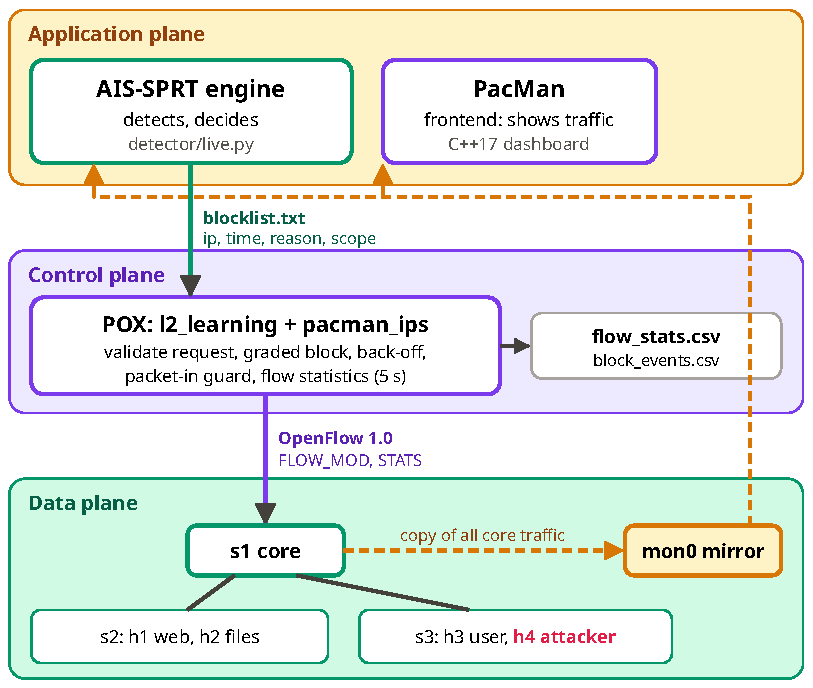
\includegraphics[width=\columnwidth]{figures/d_planes.pdf}
\caption{System architecture: mirrored observations feed the detector, and
OpenFlow enforces the selected response.}
\label{fig:architecture}
\end{figure}

The fixed comparator converts a suspicion to an immediate host block and uses a fixed timeout.
The graded comparator initially blocks only the suspected path and backs off on repeat host
decisions. Both can run with or without the guard. Scope and repeat-offence duration therefore
both vary between policies; the persistent-delivery contrast is not a scope-only effect.
The live false-suspicion fixture, by contrast, uses the same base duration and one suspicion
per trial. We make no quantitative claim about attacker identity, shared-IP attribution,
or unseen traffic beyond the mirror.

\section{Evaluation Design}
\begin{table*}[t]
\centering\small
\caption{Evidence map. Live execution, offline replay, and simulation answer different questions.}
\begin{tabular}{@{}p{.22\textwidth}p{.28\textwidth}p{.42\textwidth}@{}}
\toprule Experiment & Design & What the result supports \\
\midrule
Controlled enforcement & 80 live trials; 20 paired seeds, four policy/guard arms &
Delivery and install-time effects with the same injected decisions; not detector accuracy \\
Live false suspicion & 12 live trials; six paired seeds, equal base timeout & Collateral after a real
detector-generated error; not the population false-positive rate \\
Live HTTP fixture & Detector-driven graded, fixed, and monitor-only arms & Application-level
collateral and suppression of a designated stream; not malicious-workload or scale containment \\
Original closed loop & Four-host live lab, one implementation & Feasibility and timing on selected workloads;
not a repeated policy comparison \\
Capture feasibility & One 200-source Mininet run & Capture completeness in this run; not recall,
victim availability, or containment \\
Detector evaluation & Offline replay plus attempt-level simulation & Detection errors and sensitivity;
not live enforcement performance \\
\bottomrule
\end{tabular}
\label{tab:evidence}
\end{table*}
Table~\ref{tab:evidence} separates the evidence by experimental design. The
primary outcomes are measured packet delivery and collateral loss; barrier
acknowledgements mark installation progress, not the recovery of an application.

\section{Measured Containment--Collateral Trade-off}
We use Mininet~\cite{lantz2010mininet} in a dedicated WSL lab. Each of 20 seeds fixes the
topology and traffic parameters across four arms; arm order is randomized. A fixed sequence
of decisions isolates enforcement from detection. UDP sender sequence IDs are joined to
victim receipt logs. Initial ACK time is measured to the last switch barrier reply; it is
not application recovery time. Installation-window receipts are arrivals between the first
install-send and the last initial ACK, and can include in-flight traffic. Other-destination
collateral is the lost fraction of otherwise legitimate packets from the falsely suspected
source. Persistent delivery is the delivered fraction after the second repeat decision.
Differences are paired by seed, with percentile bootstrap 95\% intervals.
For each contrast we calculate a difference within each seed (averaging over
the other factor), then average those seed differences. The interval is
the 2.5th to 97.5th percentile of 2,000 bootstrap resamples of the seed
differences~\cite{efron1979bootstrap}. We do not resample individual packets:
packets sent under the same controller decision share a measurement window
and are not independent replications. The live pilot uses the same paired
procedure with six seeds, so its interval should be interpreted in the
context of a small, deliberately constructed workload.

\paragraph{Statistical analysis.}
Seed is the unit of analysis. For every contrast we also report the standard
deviation of the 20 seed differences, the paired standardized effect
$d_z=\bar{\Delta}/s_\Delta$, and how many seeds had a negative, zero, or
positive difference. The two-sided Wilcoxon signed-rank test~\cite{wilcoxon1945individual}
is used because the seed differences are bounded and not assumed normal; zero
differences are discarded, and $p$-values use the normal approximation when
ties are present. The ten tests in Table~\ref{tab:inference} are a single family,
and we apply the Holm step-down correction~\cite{holm1979simple} to control the
family-wise error rate at 5\%. Pooled proportions are reported with Wilson score
intervals~\cite{wilson1927probable}; because packets in one trial share a decision,
those intervals are descriptive, and inference is made on seeds. All statistics are
regenerated from the trial records by \texttt{extended\_stats.py}.

\begin{table*}[t]
\centering\small
\caption{Controlled enforcement: paired effects, mean [95\% seed-bootstrap interval].
Negative differences favor the first arm for these loss, delivery, and time metrics;
pp denotes percentage points.}
\begin{tabular}{@{}lll@{}}
\toprule Metric & First arm minus second arm & Difference \\
\midrule\PolicyEffects\bottomrule
\end{tabular}\label{tab:policy}
\end{table*}

Table~\ref{tab:policy} shows two distinct effects: grading protects unrelated connectivity,
while the guard reduces observed installation-window receipts. The initial ACK-time contrast
does not clearly favor either policy. Full-host ACK comes later with grading, as the fixed
policy already acts on suspicion. Lower persistent delivery is evidence for the policy
bundle in this workload, not evidence that grading dominates at equal block duty cycle.

The four arms help interpret the aggregate contrasts. With the guard off,
the mean number of arrivals in the initial installation window was 1.00
for fixed and 1.10 for graded blocking. With the guard on, the corresponding
means were 0.05 and 0.10. The residual is small in this test, but it is not
zero and cannot be attributed entirely to new learning. In both fixed
arms, about half of the monitored legitimate traffic to the unrelated
destination was lost after the injected false suspicion. Neither graded
arm observed that loss. This comparison concerns the unrelated destination;
it does not imply that traffic to the selected destination remained available.

\begin{table*}[t]
\centering\small
\caption{Paired inference over 20 seeds. $\Delta$: mean seed difference [95\% seed-bootstrap
interval]; $s_\Delta$: SD of seed differences; $d_z=\bar\Delta/s_\Delta$; $-/0/+$: seeds with
negative, zero, or positive difference; $p$: two-sided Wilcoxon signed-rank; $p_{\mathrm{Holm}}$:
adjusted over all ten tests.}
\begin{tabular}{@{}llrrrcrr@{}}
\toprule Metric & Contrast & $\Delta$ [95\% CI] & $s_\Delta$ & $d_z$ & $-/0/+$ & $p$ & $p_{\mathrm{Holm}}$ \\
\midrule\InferenceRows\bottomrule
\end{tabular}\label{tab:inference}
\end{table*}

\begin{table*}[t]
\centering\small
\caption{Per-arm distribution over 20 seeds: median (interquartile range). G0/G1: packet-in guard off/on.}
\begin{tabular}{@{}lllll@{}}
\toprule Metric & Fixed, G0 & Fixed, G1 & Graded, G0 & Graded, G1 \\
\midrule\ArmDescriptiveRows\bottomrule
\end{tabular}\label{tab:arms}
\end{table*}

\paragraph{Interpreting the inference.}
Table~\ref{tab:inference} separates three kinds of result. First, three policy
effects are large and consistent. Grading lowered collateral loss in all 20 seeds
($d_z\approx-10$) and lowered persistent attacker delivery in all 20. It also
delayed full-host acknowledgement in all 20 seeds. All three effects remain
significant after Holm adjustment. The size of the effect relative to the spread
across seeds means these conclusions do not depend on a few favorable runs.
Second, the guard effect on installation-window receipts is moderate
($d_z\approx-1$) and survives correction. Sixteen seeds improved, three were tied,
and one moved the wrong way. The guard reduces this exposure but does not
reliably eliminate it. Third, the remaining six contrasts are not distinguishable
from zero after correction. No clear difference was detected in initial
acknowledgement time ($-0.033$~s; 95\% CI [$-0.132$, $+0.078$]).
The interval permits both faster and slower installation under grading;
we did not test equivalence. The guard also had no detectable effect on collateral loss or
acknowledgement timing, which is consistent with its narrow role of suppressing
packet-ins and does not make its benefit depend on a slower control path.

Table~\ref{tab:arms} gives the distributions behind these contrasts. The fixed arms
have collateral interquartile ranges around 46--54\%, whereas both graded arms have
an interquartile range of exactly zero. Persistent-attacker delivery is around 72\%
under fixed blocking and 23--25\% under grading. This difference is partly caused by
graded repeat TTLs (final accepted TTL 4~s vs.\ 1~s), so it should be read as the
effect of the policy bundle rather than block scope alone.

\begin{figure*}[t]
\centering
\includegraphics[width=.47\textwidth]{\abfig{16_collateral_fraction}}
\includegraphics[width=.47\textwidth]{\abfig{20_persistent_delivery_fraction}}
\caption{Controlled enforcement: collateral to the unrelated destination and attacker delivery
after repeated decisions. These are measured receipts, not predicted from flow rules.}
\label{fig:tradeoff}
\end{figure*}

\section{Live Detector-to-Enforcement Pilot}
Six paired seeds run the actual packet tracker, AIS-SPRT process, block-request file, POX,
and OVS with the guard enabled in both arms. No decisions are injected. A benign client
has two stale TCP health-check entries on one server while sending useful datagrams to
another server. A separate benign host sends to that second server as a negative control.
This deliberately tests one false-suspicion mechanism, not the prevalence of false
positives. The controller uses the same three-second base timeout for both policies.
We verify all-switch installation ACKs and join sender and receiver records in a fixed
five-second window beginning with the health-check fixture.

\begin{table}[ht]
\centering\small
\caption{Live pilot: pooled legitimate losses / packets offered to the unaffected destination.
Statistical inference uses pairs, not individual packets.}
\begin{tabular}{@{}lrr@{}}
\toprule Policy & Suspected source & Control source \\
\midrule
Fixed & \LiveFixed \\
Graded & \LiveGraded \\
\bottomrule
\end{tabular}\label{tab:live}
\end{table}

The paired graded-minus-fixed difference in loss for the falsely suspected source is
\LiveDelta{} percentage points (95\% seed-bootstrap interval). This verifies a mechanism:
scope preserved unrelated traffic after a real detector error in this fixture.
It does not establish attack containment when the detector drives the controller, or
generalize the observed loss rates to other applications or sites.

\begin{table}[ht]
\centering\small
\caption{Live pilot by seed: lost/sent (loss \%) for the suspected source to the unaffected
destination, control-source losses over both arms, and graded$-$fixed difference (pp).}
\setlength{\tabcolsep}{4pt}
\begin{tabular}{@{}rllrr@{}}
\toprule Seed & Fixed & Graded & Control & $\Delta$ \\
\midrule\LivePairRows\bottomrule
\end{tabular}\label{tab:livepairs}
\end{table}

Table~\ref{tab:livepairs} shows that the result does not rely on a pooled average.
Fixed blocking lost between 41.5\% and 73.5\% of unrelated legitimate packets in
every pair, while graded blocking lost none. The control source lost no packets in
either arm, which makes a general path outage an unlikely explanation. The
seed differences have SD \LiveSD{}~pp and $d_z=\LiveDz{}$. With six pairs that all
have the same sign, the exact sign test and the Wilcoxon signed-rank test both give
$p=\LiveSignP{}$, the smallest value either can reach with $n=6$. The pooled loss
proportion is \LiveFixedWilson{} for fixed and \LiveGradedWilson{} for graded
(Wilson 95\% intervals); these are descriptive because packets within a pair are not
independent. The variation in fixed-arm loss between pairs reflects when the host
rule took effect relative to the client's sending schedule, not variation in the
graded arm.

\section{Matched-Duration Live Service Comparison}
\label{sec:live-service}
We add an application-level test to distinguish actual transaction failures from
lost UDP datagrams. Two retired health checks trigger suspicion in a live
Mininet/OVS/POX network. The flagged client then issues ordinary HTTP requests to
both the selected destination and an unrelated service. An independent client
queries the unrelated service as a negative control. The selected stream is
designated for suppression in this test; it is harmless and does not model an
attack. The two enforcement arms use the same configured five-second first-action
timeout and enable the guard. The monitor-only arm runs the same detector but
does not pass its requests to the controller. No decisions are injected.

Each stream offers 16 HTTP requests at four per second. Legitimate request
success requires a client-observed HTTP 204 response; the socket timeout is
150\,ms. Containment by two seconds means no selected-stream request reached
the server at or after two seconds from the scheduled stale-check onset,
through the end of the fixture. The server log, not a missing client response
or a switch barrier, determines target receipt. The test stops within the
configured first-action window; it does not measure recurrence after expiry.

\begin{table*}[t]
\centering\small
\caption{Live HTTP fixture on 20 randomized seed blocks per arm. Alert counts
refer to the expected suspicion; installation counts require all switch ACKs.}
\begin{tabular}{@{}lrrrrrr@{}}
\toprule Arm & Alert trials & Installed trials & Target received & Unrelated succeeded &
Control succeeded & Contained by 2\,s \\
\midrule\ServiceRows\bottomrule
\end{tabular}\label{tab:service}
\end{table*}
\begin{table}[ht]
\centering\small
\caption{Matched HTTP fixture: paired mean differences in percentage points
[95\% seed-bootstrap interval].}
\resizebox{\columnwidth}{!}{%
\begin{tabular}{@{}lll@{}}
\toprule Contrast & Outcome & Difference \\
\midrule\ServiceDiffs\bottomrule
\end{tabular}}\label{tab:servicediff}
\end{table}
Table~\ref{tab:service} reports all trials, not only those that alerted or
installed a rule. Table~\ref{tab:servicediff} reports differences within the
same topology seed (4101--4120), with randomized arm order. Equal configured
timeouts do not imply equal arrival-to-install delays. The fixed--graded
contrast separates the first action from the repeat-offence schedule.

Grading improved unrelated request success by 89.1 percentage points
over fixed blocking (95\% interval [85.3, 92.5]), but did not recover
the monitor-only success rate. Both blocking arms delivered 27 of 320
selected requests before the deadline, compared with 320 of 320 under
monitoring. The paired receipt difference was 0.0 percentage points
[$-4.1$, $+4.1$]; this does not establish equivalence. Both blocking
arms met the two-second criterion in all 20 seeds, compared with none
under monitoring. The independent control also missed some requests in
both blocking arms; these data do not identify the cause of those misses.

In an earlier development attempt, no arm generated a suspicion with the
connectivity checks running under detector observation. The final protocol
moves preflight before detector startup. Neither development run contributes
to the prespecified campaign.

\paragraph{Where scope helps and where it fails.}
The relevant benefit is preservation of transactions from the flagged client
to a different destination, not preservation of every legitimate request.
A path block also suppresses legitimate requests to the selected destination.
It cannot suppress harmful traffic to other destinations before escalation.
Conversely, no action preserves access but offers no suppression. This fixture
tests the first action on one destination with offered load below saturation;
it does not establish an availability benefit or containment for a malicious
or distributed workload.

\section{Detector Evidence and Its Limits}
The attempt simulator uses 12 training, eight validation, and 20 held-out seeds. It
randomizes workload and propagation delay. Recorded edge assignments are metadata,
not inputs to delay, queueing, or forwarding. Logical sources are not independent
namespaces. Scripted adaptive workloads expose policy risks but do not represent
live attackers reacting to enforcement.

RF features are bucketed by outcome availability, not start time, so an offline
window cannot observe a future outcome. The training fit omits windows that
straddle known onset; prediction does not depend on labels. Validation selects
operating points before testing. These are not matched-FPR comparisons: use the
observed operating points to interpret the precision/recall trade-off, not to
claim a universal ranking. Bootstrapping resamples seeds. An all-zero estimated
interval is not a proof of zero risk.

The Random Forest~\cite{breiman2001random} uses 200 trees and six features
computed over ten-second windows: count, distinct destinations, distinct
destination services, observed failure fraction, destination-port entropy,
and resolved-attempt rate. The selected model has maximum depth eight,
minimum leaf size one, and an alarm threshold of 0.5. For AIS-SPRT the
selected simulation settings are $\alpha=0.01$, $\tau=600$\,s, and flood
threshold $h=620$. Training seeds are 1--12, validation seeds 1001--1008,
and test seeds 2001--2020. Test runs are not used to select the thresholds.
Selection first prefers candidates whose validation false-positive rate is
at most 1\%, then higher F1 and lower false-positive rate. The selected RF
had a validation false-positive rate of 2.34\%; the preference is not a
hard constraint or a deployment guarantee.

The confusion table pools host-runs; the interval table gives each seed
equal weight after averaging the scenarios for which the metric is defined.
Those denominators answer
different questions: large distributed scenarios can dominate the pooled
count while contributing only one scenario to a seed average. Observed
zero confirmed false positives for tuned AIS-SPRT does not imply absence
of false suspicion. Conversely, RF's higher macro F1 comes with a nonzero
confirmed false-positive rate. A comparison intended to choose a deployment
threshold would need independent validation at a common collateral or
false-alarm budget, not selection from these test results.

\begin{table*}[t]
\centering\small
\caption{Held-out attempt simulation: pooled host-run confusion counts; seed-macro F1,
precision, 10-second recall (misses count as failures), and benign suspicion rate.
Precision omits scenarios with no positive prediction. Suspicion is an additional AIS action
and is distinct from a confirmed false alarm.}
\begin{tabular}{@{}lrrrrrrrr@{}}
\toprule Method & TP & FN & FP & TN & F1 & Precision & Recall $\le 10$s & Suspicion FPR \\
\midrule\DetectorRows\bottomrule
\end{tabular}\label{tab:confusion}
\end{table*}

\begin{table*}[t]
\centering\small
\caption{Selected detector operating points: seed-macro means [95\% seed-bootstrap interval].
F1 averages attack scenarios only; FPR includes benign scenarios.}
\begin{tabular}{@{}llll@{}}
\toprule Method & F1 & Recall & Confirmed FPR \\
\midrule\DetectorIntervals\bottomrule
\end{tabular}\label{tab:detectors}
\end{table*}

\begin{table}[ht]
\centering\small
\caption{Pooled host-run detection rates with Wilson 95\% intervals (descriptive; host-runs
within a seed are correlated).}
\setlength{\tabcolsep}{3pt}
\begin{tabular}{@{}llll@{}}
\toprule Method & TPR & Confirmed FPR & Prec. \\
\midrule\DetectorWilsonRows\bottomrule
\end{tabular}\label{tab:wilson}
\end{table}

\begin{table}[ht]
\centering\small
\caption{Paired seed-level detector contrasts over 20 test seeds: mean [95\% bootstrap
interval], $d_z$, seeds where RF is higher, and Wilcoxon $p$.}
\setlength{\tabcolsep}{2.5pt}
\resizebox{\columnwidth}{!}{%
\begin{tabular}{@{}llllrr@{}}
\toprule Metric & Pair & $\Delta$ [95\% CI] & $d_z$ & RF$>$ & $p$ \\
\midrule\DetectorPairRows\bottomrule
\end{tabular}}\label{tab:detpairs}
\end{table}

Tables~\ref{tab:wilson} and~\ref{tab:detpairs} show that the detector ranking is a
trade-off, not a winner. At the selected operating points, RF had higher F1 and
recall than tuned AIS-SPRT and TRW in every test seed. It also had a higher confirmed
false-positive rate in every seed, about 1.9\% of benign host-runs against
no observed confirmed false positives for tuned AIS-SPRT. This comparison is
secondary: RF was not connected to the live controller, the test operating points
were not matched on false-positive rate, and the extra RF confirmations cannot be
translated into a measured service cost. Tuned AIS can also act on a suspicion
without confirming it. Very large $d_z$ values for recall reflect nearly constant
per-seed differences, not a practically larger effect, and should not be compared
with the enforcement effect sizes. Because the operating points were not matched on
false-positive rate, these contrasts compare the selected systems rather than the
underlying models.

The classical Wald probability bound~\cite{wald1945sequential} applies only to one
unmodified stopped test under the specified independent likelihood model.
It is not a lifetime bound after resets, weights, decay, or a separate rate alarm.
Appendix~\ref{app:boundary} checks the separate analytic slow-rate prediction under its stated
assumptions. Finite TTL and capacity eviction can discard evidence. Defaults cap
state at 4,096 sources, 65,536 scored contacts, and 16,384 service entries, with
3,600~s aging and bounded memberships; these are entry caps, not RSS guarantees.

A separate 30\,s run exercised \ScaleSources{} real source namespaces and
recorded \ScalePackets{} packets and \ScaleAttempts{} resolved attempts, with
zero reported kernel capture drops. That establishes feasibility of capture,
not detector recall or containment. The full train/validation/test campaign at
that scale was not run. Appendix~\ref{app:historical} reports the earlier
Mininet and CIC-IDS2017 results~\cite{sharafaldin2018cicids}, including false
alarms and a failed timing check. These historical results do not justify
selecting a deployment threshold on the test capture.

\section{Limitations and Next Evaluation}
\paragraph{Internal validity.}
Controlled trials use the same request sequence in each paired arm, but do
not isolate block scope from the repeat-offence schedule. The six-pair live
pilot isolates the first action at the same base timeout, but only for one
constructed false-suspicion mechanism. Neither result estimates how often a
production workload will trigger that mechanism.

\paragraph{Measurement and external validity.}
The measured guard effect is from a small, isolated testbed and does not
guarantee zero leakage. A barrier reply does not demonstrate that a rule
preserved application availability, and sequence-matched UDP delivery does
not measure completed application transactions. Timing also depends on
request polling, controller and host scheduling, switch processing, and
topology. The trace study does not establish transfer across sites, and the
simulator does not capture feedback between enforcement and subsequent
traffic. Shared addresses can also expand the impact of a host-level action
beyond the endpoint that generated the evidence.

\paragraph{Next evaluation.}
Hold out whole workloads or sites and freeze the detector's operating point
on validation. Compare live policies under a matched timeout or measured
block-time budget. Measure successful victim requests, legitimate goodput,
and containment by a prespecified deadline in addition to collateral.
Report the paired outcomes for cases where a path action preserves service
and for cases where it leaves other destinations exposed. The matched first-action HTTP fixture does not establish repeat-offence
behavior under a matched block-time budget or large-scale containment.

\section{Reproducibility}
The accompanying artifact includes seed and configuration manifests for the
expanded simulation, raw sender and receiver records with switch barrier
traces for the controlled trials, detector requests and packet receipt
records for the live pilot, and HTTP client outcomes and server receipt logs
for the matched first-action fixture. The analysis scripts derive policy contrasts from
paired seed results and regenerate the detector tables from host-run records.
Historical replay tables are retained separately; rerunning the corrected
windowed RF pipeline on a new workload does not revise those historical
measurements automatically.

\section{Conclusion}
An enforcement evaluation must measure who actually lost connectivity and when,
not just whether the detector alarmed. The controlled trials quantify the
containment--collateral trade-off, and the live pilot reproduces the collateral
mechanism for an actual false suspicion. Those findings support graded responses
in the tested conditions without requiring a claim of universal detection
superiority.

Quantitatively, three policy effects held in every one of 20 paired seeds and
survived Holm correction. Grading reduced collateral loss by about 50~pp and
persistent attacker delivery by about 48~pp, but delayed the full-host ACK by about
0.68~s. In the live pilot, all six pairs favored grading. No clear difference was
detected in time to the first rule. The packet-in guard reduced, but did not
eliminate, installation-window exposure. In the matched HTTP fixture,
grading preserved substantially more unrelated transactions than fixed
blocking, while both suppressed the selected stream by the deadline.
The fixture does not measure collateral
at the selected destination under legitimate load or establish containment
across destinations. These are the next outcomes to test under a matched
repeat-block budget.

\appendices
\section{Detector Model and Slow-Rate Boundary}\label{app:boundary}
For source $s$, the detector scores the first observed outcome to a
destination service within the contact retention horizon. For each such
outcome it updates $L\leftarrow e^{-\Delta/\tau}L+x$, where
$x=\ln(\theta_1/\theta_0)$ for success and
$x=w\ln((1-\theta_1)/(1-\theta_0))$ for failure. The default success
probabilities are $\theta_0=0.8$ and $\theta_1=0.2$; $\tau=600$\,s.
The popularity weight is $w=\max(0.25,1/(1+n))$, where $n$ counts other
remembered sources for the service. With nominal $\alpha=0.01$ and
$\beta=0.99$, the confirmation boundary is $\eta=\ln(\beta/\alpha)$,
and suspicion starts at $\eta/2$. These parameters are score settings,
not deployed error guarantees.

For periodic failed contacts with unused services, weight one, no resets
before the first alarm, and no eviction, $L_n=c+e^{-\Delta/\tau}L_{n-1}$.
Starting at zero, its limit is $c/(1-e^{-\Delta/\tau})$. With $0<c<\eta$,
the score crosses $\eta$ in finite time only when this limit exceeds $\eta$.
Fig.~\ref{fig:slow-integrated} compares the predicted boundary with nine
detector runs. Runs stop at first alarm or five hours; observed peaks on
detected runs stop at crossing. This is a deterministic implementation
check rather than a stochastic detection probability.

\begin{figure}[!t]
\centering
\includegraphics[width=\columnwidth]{\simfig{15_slow_boundary}}
\caption{Analytical and observed score near the slow-rate boundary.}
\label{fig:slow-integrated}
\end{figure}

\section{Additional Detector and Enforcement Results}
\newcommand{\simpanel}[1]{\includegraphics[width=.47\textwidth]{\simfig{#1}}}
\newcommand{\abpanel}[1]{\includegraphics[width=.47\textwidth]{\abfig{#1}}}
\begin{figure*}[!t]
\centering
\simpanel{01_F1_ci}\simpanel{02_FPR_ci}\\
\simpanel{03_scenario_TPR}\simpanel{04_scenario_FPR}\\
\simpanel{05_delay}\simpanel{06_RF_pr}
\caption{Held-out attempt simulation: operating points, scenario errors,
conditional delay, and the descriptive RF precision--recall curve.
Misses are reflected in recall, not in the delay distribution.}
\end{figure*}

\begin{figure*}[!t]
\centering
\simpanel{07_padding}\simpanel{08_sources}\\
\simpanel{09_failure}\simpanel{10_tau}
\caption{Synthetic workload and parameter sensitivity. Source counts here
are logical, not independently emulated host namespaces.}
\end{figure*}

\begin{figure*}[!t]
\centering
\simpanel{11_bound_H0}\simpanel{12_bound_H1}\\
\simpanel{13_memory}\simpanel{14_throughput}
\caption{Classical single-test reference, restart and weighted/decayed
simulations, and bounded-state diagnostics. The weighted recurrence does
not model learned popularity. Memory is traced allocation, not peak RSS;
throughput is instrumented attempt processing, not packet ingestion.}
\end{figure*}

\begin{figure*}[!t]
\centering
\abpanel{15_leaked_installation_packets}\abpanel{17_decision_to_initial_ack_s}\\
\abpanel{18_host_block_from_attack_start_s}\abpanel{19_last_block_duration_s}
\caption{Controlled enforcement diagnostics from the same 80 trials as
Fig.~\ref{fig:tradeoff}. Accepted TTL is a policy setting, not a delivery measurement.}
\end{figure*}

\section{Historical Evidence and Negative Results}\label{app:historical}
The original small-trace test found 16/16 detections and zero false alarms
over 176 benign host-runs for AIS-SPRT. TRW detected 14/16 and falsely
flagged 1/176. The historical offline CIC-IDS2017 Friday replay found
2/2 episodes detected but 2/8 benign hosts falsely flagged with the
morning-calibrated flood setting. Using the original emulation flood
setting increased the false count to 5/8. The scan and flood were observed
from one apparent source address; this is not multi-source validation.
These are historical outcomes, not held-out results of the updated
causal RF pipeline. A threshold sweep on the same CIC capture is
descriptive and does not justify a deployment threshold.

In the original four-host live loop, full-host rules appeared on all
three switches 0.68--1.39\,s after onset across four fast trials, and a
single slower trial was blocked after 20.2\,s. One of nine checks failed
because polling could not separate the path and host stages. These
measurements show that the original live loop could act, not that it met
a deadline or that a fixed-policy baseline would have acted later.

The expanded causal evaluation supersedes the older simulation comparison.
Tuned AIS-SPRT observed no confirmed false alarms but still generated
benign suspicions and missed many positives
(Tables~\ref{tab:confusion} and~\ref{tab:detectors}). RF had higher
macro F1 but nonzero false alarms, and the two methods were not matched
on false-positive rate. Keeping these negative outcomes visible is
essential when detector outputs can interrupt service.


\clearpage
\balance
\bibliographystyle{IEEEtran}
\bibliography{refs}
\end{document}
